\documentclass[12pt,a4paper]{article}

\usepackage[utf8]{inputenc}
\usepackage[T1]{fontenc}
\usepackage{mathptmx}
\usepackage{geometry}
\usepackage{graphicx}
\usepackage{booktabs}
\usepackage{multirow}
\usepackage{array}
\usepackage{amsmath}
\usepackage{amssymb}
\usepackage{float}
\usepackage{caption}
\usepackage{subcaption}
\usepackage{xcolor}
\usepackage{hyperref}
\usepackage{enumitem}
\usepackage{longtable}
\usepackage{setspace}
\usepackage{indentfirst}
\usepackage{titlesec}
\usepackage{tocloft}

\geometry{
    left=3.0cm,
    right=2.0cm,
    top=2.5cm,
    bottom=2.5cm
}

\graphicspath{{figs/}{figs/notebook/}}
\onehalfspacing
\setlength{\parskip}{0.15em}
\setlength{\parindent}{1.25cm}

\renewcommand{\contentsname}{TABLE OF CONTENTS}
\renewcommand{\listfigurename}{LIST OF FIGURES}
\renewcommand{\listtablename}{LIST OF TABLES}
\renewcommand{\figurename}{Figure}
\renewcommand{\tablename}{Table}

\titleformat{\section}
  {\normalfont\Large\bfseries\centering}
  {\thesection}{1em}{\MakeUppercase}
\titleformat{\subsection}
  {\normalfont\large\bfseries}
  {\thesubsection}{1em}{}
\titleformat{\subsubsection}
  {\normalfont\normalsize\bfseries}
  {\thesubsubsection}{1em}{}

\titlespacing*{\section}{0pt}{1.5em}{1.0em}
\titlespacing*{\subsection}{0pt}{1.0em}{0.4em}
\titlespacing*{\subsubsection}{0pt}{0.8em}{0.3em}

\captionsetup{
    font=small,
    labelfont=bf,
    justification=centering
}

\setlist[itemize]{leftmargin=1.2cm, itemsep=0.15em, topsep=0.2em}
\setlist[enumerate]{leftmargin=1.2cm, itemsep=0.15em, topsep=0.2em}

\hypersetup{
    colorlinks=true,
    linkcolor=black,
    citecolor=black,
    urlcolor=black
}

\newcommand{\projecttitle}{Credit Card Fraud Detection}
\newcommand{\reportauthor}{Nguyen Huy Minh}
\newcommand{\classname}{AI66A}
\newcommand{\university}{National Economics University}
\newcommand{\supervisor}{Dr. Thien Van Luong}
\newcommand{\reportdate}{Hanoi, May 2026}
\newcommand{\frontsection}[1]{%
    \section*{\centering #1}%
    \addcontentsline{toc}{section}{#1}%
}

\begin{document}

% ============================================================
% COVER PAGE
% ============================================================
\begin{titlepage}
    \centering
    {\large \textbf{NATIONAL ECONOMICS UNIVERSITY}}\\
    {\large \textbf{SCHOOL OF TECHNOLOGY}}\\[2.2cm]

    {\Large \textbf{REPORT}}\\[0.35cm]
    {\large \textbf{STATISTICAL LEARNING}}\\[1.7cm]

    \begin{flushleft}
    \hspace{1.5cm}\textbf{Topic:} \MakeUppercase{\projecttitle}\\[0.35cm]
    \hspace{1.5cm}\textbf{Focus:} XGBoost, Feature Selection, and Drift-Aware Evaluation\\[0.35cm]
    \hspace{1.5cm}\textbf{Student:} \reportauthor\\[0.35cm]
    \hspace{1.5cm}\textbf{Class:} \classname\\[0.35cm]
    \hspace{1.5cm}\textbf{Supervisor:} \supervisor
    \end{flushleft}

    \vfill
    {\large \reportdate}
\end{titlepage}

\pagenumbering{roman}

% ============================================================
% PREFACE
% ============================================================
\frontsection{PREFACE}

In modern digital finance, electronic payments and online transactions provide strong convenience for users but also create a large attack surface for fraudulent activities. Credit card fraud is particularly challenging because fraudulent transactions are rare, heterogeneous, and often designed to look similar to legitimate behavior. A detection system must therefore satisfy two competing requirements: it must catch as many fraudulent transactions as possible, while avoiding excessive false alerts that inconvenience legitimate customers.

This project investigates the use of machine learning for credit card fraud detection on a large-scale tabular transaction dataset. The work focuses on exploratory data analysis, feature engineering, feature selection, class imbalance handling, XGBoost model training, threshold optimization, and drift-aware evaluation across time-sorted data chunks. The final analysis shows that strong performance on a single chunk is not sufficient: later chunks reveal both concept-like drift and threshold calibration drift, making temporal validation essential.

The report is organized as a complete machine learning project: it first defines the problem and data, then describes the preprocessing and modeling pipeline, reports experimental results, analyzes chunk-level generalization, and finally proposes a practical deployment and monitoring plan.

\newpage

% ============================================================
% DECLARATION
% ============================================================
\frontsection{DECLARATION}

I hereby declare that the content presented in this report is the result of my own learning, implementation, analysis, and project work. The experiments, figures, tables, and conclusions are based on the project notebook \texttt{Data\_fraud.ipynb}, the generated result files, and the model evaluation outputs obtained during the project.

All external concepts and algorithms mentioned in this report, including XGBoost, Random Forest, class imbalance learning, and evaluation metrics, are cited in the References section. I take responsibility for the honesty and integrity of the analysis presented in this report.

\vspace{1.0cm}
\begin{flushright}
\reportdate\\
Declarant\\[1.0cm]
\textbf{\reportauthor}
\end{flushright}

\newpage

\tableofcontents
\newpage
\listoffigures
\newpage
\listoftables
\newpage

% ============================================================
% ABBREVIATIONS
% ============================================================
\frontsection{ABBREVIATIONS}

\begin{table}[H]
\centering
\begin{tabular}{ll}
\toprule
\textbf{Abbreviation} & \textbf{Full Form} \\
\midrule
AI & Artificial Intelligence \\
ML & Machine Learning \\
EDA & Exploratory Data Analysis \\
RF & Random Forest \\
XGBoost & Extreme Gradient Boosting \\
PR-AUC & Area Under the Precision--Recall Curve \\
ROC-AUC & Area Under the Receiver Operating Characteristic Curve \\
TP & True Positive \\
FP & False Positive \\
TN & True Negative \\
FN & False Negative \\
F1 & Harmonic mean of precision and recall \\
MI & Mutual Information \\
PSI & Population Stability Index \\
\bottomrule
\end{tabular}
\end{table}

\newpage

% ============================================================
% ABSTRACT
% ============================================================
\frontsection{ABSTRACT}

This report presents a credit card fraud detection project using tree-based machine learning models, with XGBoost as the final modeling approach. The dataset is highly imbalanced: in the first time-sorted chunk used for detailed exploratory analysis, fraudulent transactions account for only 1.0597\% of all transactions. Because of this imbalance, accuracy is not a reliable evaluation metric; instead, the project uses PR-AUC, precision, recall, F1-score, and confusion matrix analysis.

Exploratory data analysis shows that transaction amount and category are the strongest fraud signals, while distance between customer and merchant and time-of-day have weak standalone predictive power. Feature selection reduces the model-ready feature set from 41 features to 25 features with almost no loss in PR-AUC. XGBoost models are trained under different imbalance-handling strategies. On data chunk 01, both tuned XGBoost candidates achieve strong test performance, with PR-AUC above 0.96 and F1-score above 0.95.

However, evaluating later chunks reveals that strong chunk-01 performance does not guarantee stable generalization. Some chunks show true ranking degradation, while others show low F1-score despite high PR-AUC, indicating threshold calibration drift rather than concept drift. The final recommendation is to use \texttt{xgb\_class\_weight} as the production baseline, combined with dynamic thresholding, walk-forward validation, and drift monitoring.

\newpage
\pagenumbering{arabic}

% ============================================================
\section{Problem Definition}
% ============================================================

\subsection{Rationale of the Project}

Credit card fraud detection is a critical application of machine learning in financial security. In a real transaction stream, fraudulent behavior is rare but costly. A trivial classifier that predicts every transaction as legitimate can achieve very high accuracy, yet it fails completely from a risk-management perspective. Therefore, fraud detection must be evaluated using metrics that focus on the minority class and reflect operational trade-offs.

The project aims to build a model that can identify fraudulent transactions using transaction attributes, customer behavior features, merchant-related features, and time-based information. The key challenge is to balance fraud recall with false alert control. Missing fraud cases creates financial loss, while over-flagging legitimate transactions damages customer experience and increases operational cost.

\subsection{Problem Statement}

Let each transaction be represented by a feature vector $\mathbf{x}_i$ and binary target $y_i \in \{0,1\}$, where $y_i=1$ indicates fraud. The objective is to learn a model $f(\mathbf{x}_i)$ that outputs a fraud probability:
\begin{equation}
    \hat{p}_i = f(\mathbf{x}_i) = P(y_i = 1 \mid \mathbf{x}_i).
\end{equation}

A decision threshold $\tau$ is then applied:
\begin{equation}
    \hat{y}_i =
    \begin{cases}
        1, & \hat{p}_i \ge \tau,\\
        0, & \hat{p}_i < \tau.
    \end{cases}
\end{equation}

The model must perform well not only on the first training chunk but also across future time-sorted chunks. This makes temporal validation and drift analysis important parts of the project.

\subsection{Why Fraud Detection Is Hard}

The main difficulties observed in this project are:
\begin{itemize}
    \item \textbf{Severe class imbalance}: fraud is only about 1\% of transactions.
    \item \textbf{Non-linear feature interactions}: category, amount, job, and customer behavior interact in non-linear ways.
    \item \textbf{Potential dataset artifacts}: some categories appear nearly deterministic in chunk 01.
    \item \textbf{Temporal instability}: later chunks show different behavior from chunk 01.
    \item \textbf{Threshold sensitivity}: F1-score can collapse if the validation threshold is no longer suitable for future data.
\end{itemize}

% ============================================================
\section{Data Overview}
% ============================================================

\subsection{Data Source and Chunking}

The project uses a large credit card transaction dataset stored in parquet chunks. The full processed dataset contains 16 time-sorted chunks. Each chunk contains approximately 536K transactions. The detailed EDA and initial model tuning are performed on chunk 01, while chunks 02--16 are used for cross-chunk validation and drift analysis.

\begin{table}[H]
\centering
\caption{Overall dataset summary}
\begin{tabular}{lr}
\toprule
\textbf{Attribute} & \textbf{Value} \\
\midrule
Total transactions & 8,580,255 \\
Fraud transactions & 94,806 \\
Overall fraud rate & 1.105\% \\
Number of time-sorted chunks & 16 \\
Rows per chunk & $\approx$ 536K \\
Evaluated future chunks & 02--16 \\
\bottomrule
\end{tabular}
\end{table}

\subsection{Chunk 01 Summary}

Chunk 01 contains 536,266 transactions and 44 raw columns. It has no missing values across all columns. Important column groups include identifiers, time information, transaction amount, customer profile attributes, merchant attributes, rolling customer behavior, rolling merchant behavior, and the binary target variable \texttt{is\_fraud}.

\begin{table}[H]
\centering
\caption{Chunk 01 data quality summary}
\begin{tabular}{lr}
\toprule
\textbf{Attribute} & \textbf{Value} \\
\midrule
Rows & 536,266 \\
Columns & 44 \\
Missing values & 0 \\
Unique transaction IDs & 536,266 \\
Unique accounts/cards & 8,757 \\
Unique merchants & 655 \\
Unique jobs & 639 \\
Unique categories & 14 \\
Transaction period & 2022-05-06 to 2022-05-30 \\
\bottomrule
\end{tabular}
\end{table}

\subsection{Target Variable}

The target variable is \texttt{is\_fraud}. In chunk 01, fraud accounts for only 1.0597\% of transactions.

\begin{table}[H]
\centering
\caption{Target distribution in chunk 01}
\begin{tabular}{lrr}
\toprule
\textbf{Class} & \textbf{Count} & \textbf{Rate} \\
\midrule
Non-fraud & 530,583 & 98.9403\% \\
Fraud & 5,683 & 1.0597\% \\
\bottomrule
\end{tabular}
\end{table}

\begin{figure}[H]
\centering
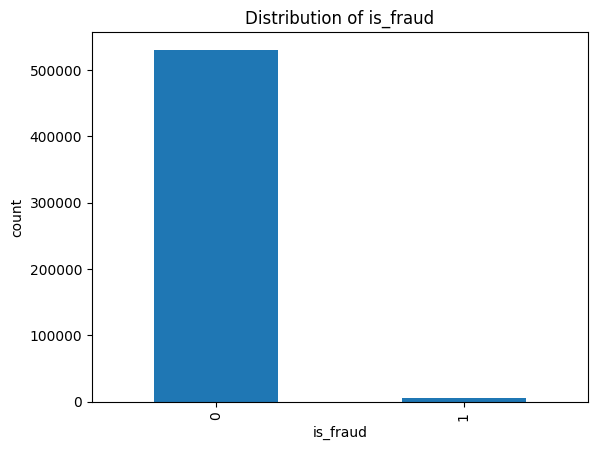
\includegraphics[width=0.55\textwidth]{cell_16_img_01.png}
\caption{Target distribution in chunk 01}
\end{figure}

This confirms that accuracy should not be used as the main metric. A classifier predicting all transactions as non-fraud would still achieve nearly 99\% accuracy, while failing to detect all fraud cases.

% ============================================================
\section{Exploratory Data Analysis}
% ============================================================

\subsection{Time-Based Analysis}

The transaction period of chunk 01 covers May 2022. The age range of customers is 14--95, with a median age of 41. Fraud rate by hour does not show a strong concentration at night, which contradicts a common heuristic that fraudulent transactions are mostly nocturnal.

\begin{figure}[H]
\centering
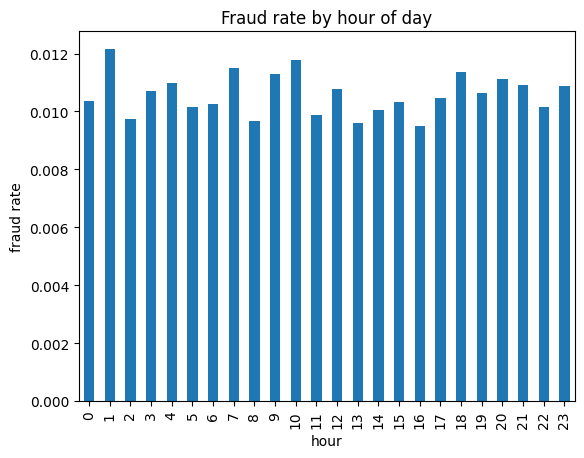
\includegraphics[width=0.70\textwidth]{cell_23_img_01.png}
\caption{Fraud rate by transaction hour}
\end{figure}

Weekend behavior is more informative. In chunk 01, weekday transactions have a higher fraud rate than weekend transactions.

\begin{table}[H]
\centering
\caption{Fraud rate by weekday/weekend in chunk 01}
\begin{tabular}{lrrr}
\toprule
\textbf{Segment} & \textbf{Total} & \textbf{Fraud} & \textbf{Fraud rate} \\
\midrule
Weekday & 285,937 & 3,778 & 1.3213\% \\
Weekend & 250,329 & 1,905 & 0.7610\% \\
\bottomrule
\end{tabular}
\end{table}

\begin{figure}[H]
\centering
\begin{subfigure}{0.48\textwidth}
    \centering
    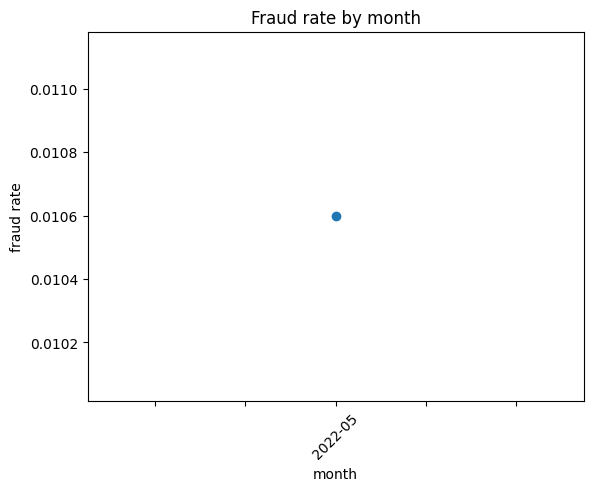
\includegraphics[width=\textwidth]{cell_27_img_01.png}
    \caption{Fraud rate by month}
\end{subfigure}
\begin{subfigure}{0.48\textwidth}
    \centering
    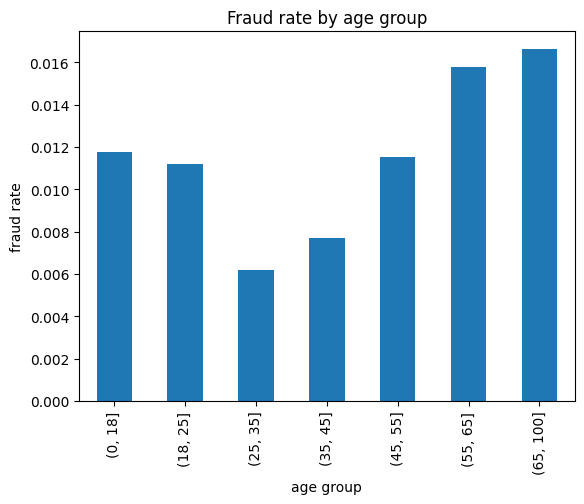
\includegraphics[width=\textwidth]{cell_29_img_01.png}
    \caption{Fraud rate by age bin}
\end{subfigure}
\caption{Time and age-related fraud patterns}
\end{figure}

The age-bin analysis suggests that older groups have higher fraud rates in chunk 01, particularly the 55--65 and 65--100 age ranges. This motivates using \texttt{age\_bin\_ord} rather than only raw age.

\subsection{Categorical Analysis}

Categorical columns have different cardinalities. Category and gender are low-cardinality variables, while merchant and job are high-cardinality variables.

\begin{table}[H]
\centering
\caption{Categorical column summary}
\begin{tabular}{lrrr}
\toprule
\textbf{Column} & \textbf{Unique values} & \textbf{Null count} & \textbf{Encoding choice} \\
\midrule
gender & 2 & 0 & Binary encoding \\
category & 14 & 0 & One-hot encoding \\
merchant & 655 & 0 & Frequency encoding \\
job & 639 & 0 & Frequency encoding \\
\bottomrule
\end{tabular}
\end{table}

Category is one of the strongest signals in chunk 01. Several categories appear to have a fraud rate of 100\%, which is useful for prediction but must be treated carefully because it may reflect a dataset artifact.

\begin{table}[H]
\centering
\caption{Selected category fraud rates in chunk 01}
\begin{tabular}{lrrr}
\toprule
\textbf{Category} & \textbf{Total} & \textbf{Fraud} & \textbf{Fraud rate} \\
\midrule
grocery\_pos & 1,394 & 1,394 & 100.0\% \\
shopping\_net & 1,299 & 1,299 & 100.0\% \\
misc\_net & 744 & 744 & 100.0\% \\
shopping\_pos & 659 & 659 & 100.0\% \\
gas\_transport & 458,338 & 465 & 0.1015\% \\
grocery\_net & 72,804 & 94 & 0.1291\% \\
\bottomrule
\end{tabular}
\end{table}

Gender has only a small difference: male transactions have a fraud rate of 1.112\%, while female transactions have a fraud rate of 1.008\%. Job is more informative than gender and merchant identity. Some job groups show fraud rates several times larger than the global baseline.

\begin{table}[H]
\centering
\caption{Top job fraud rates in chunk 01}
\begin{tabular}{lr}
\toprule
\textbf{Job} & \textbf{Fraud rate} \\
\midrule
Scientist, product/process development & 9.82\% \\
Systems developer & 7.00\% \\
Theatre manager & 6.38\% \\
Copywriter, advertising & 5.99\% \\
Holiday representative & 5.42\% \\
\bottomrule
\end{tabular}
\end{table}

\subsection{Numeric Analysis}

Transaction amount is the strongest numeric feature. Fraudulent transactions are much larger on average than legitimate transactions.

\begin{table}[H]
\centering
\caption{Selected numeric comparison between non-fraud and fraud}
\begin{tabular}{lrrrr}
\toprule
\textbf{Feature} & \textbf{Non-fraud mean} & \textbf{Fraud mean} & \textbf{Non-fraud median} & \textbf{Fraud median} \\
\midrule
amt & 78.57 & 534.61 & 61.51 & 389.44 \\
trans\_time\_hrs & 11.50 & 11.48 & 12.00 & 11.00 \\
trans\_date\_is\_weekend & 0.468 & 0.335 & 0.00 & 0.00 \\
merchant\_risk\_30\_day & 16.12 & 16.25 & 17.00 & 17.00 \\
customer\_num\_trans\_30\_day & 13.00 & 13.04 & 13.00 & 13.00 \\
\bottomrule
\end{tabular}
\end{table}

\begin{figure}[H]
\centering
\begin{subfigure}{0.48\textwidth}
    \centering
    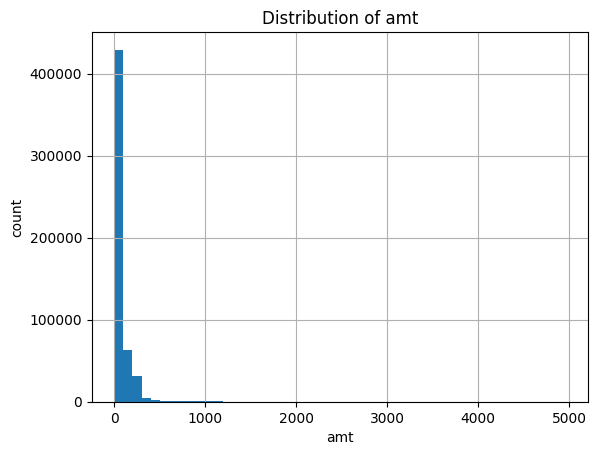
\includegraphics[width=\textwidth]{cell_44_img_01.png}
    \caption{\texttt{amt}}
\end{subfigure}
\begin{subfigure}{0.48\textwidth}
    \centering
    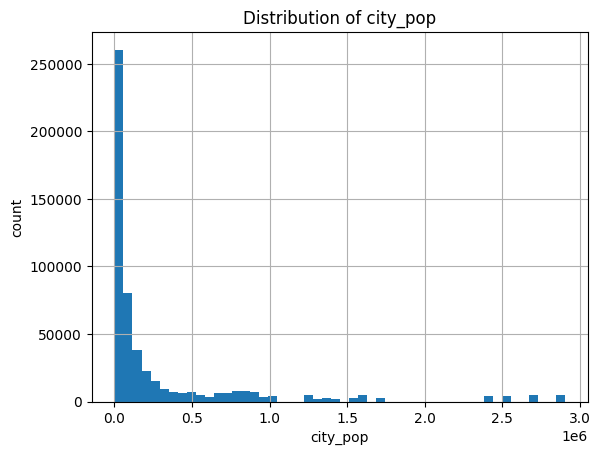
\includegraphics[width=\textwidth]{cell_44_img_02.png}
    \caption{\texttt{city\_pop}}
\end{subfigure}
\caption{Numeric distributions I}
\end{figure}

\begin{figure}[H]
\centering
\begin{subfigure}{0.48\textwidth}
    \centering
    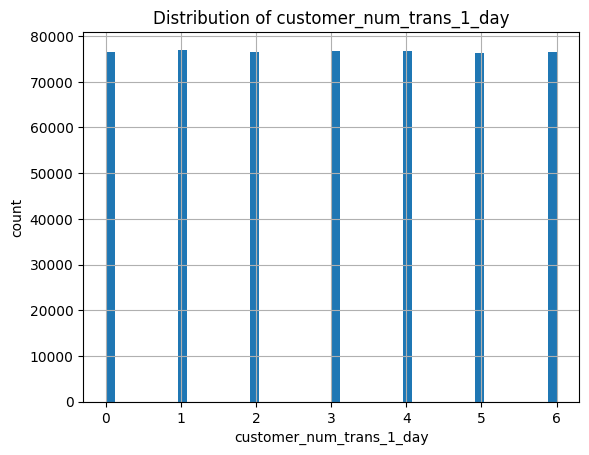
\includegraphics[width=\textwidth]{cell_44_img_03.png}
    \caption{\texttt{customer\_num\_trans\_1\_day}}
\end{subfigure}
\begin{subfigure}{0.48\textwidth}
    \centering
    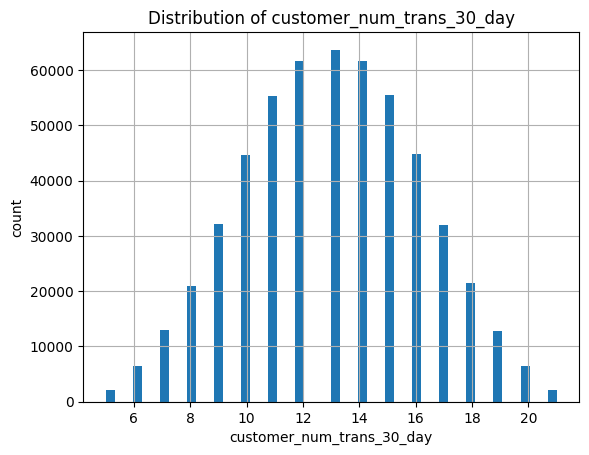
\includegraphics[width=\textwidth]{cell_44_img_04.png}
    \caption{\texttt{customer\_num\_trans\_30\_day}}
\end{subfigure}
\caption{Numeric distributions II}
\end{figure}

\begin{figure}[H]
\centering
\begin{subfigure}{0.32\textwidth}
    \centering
    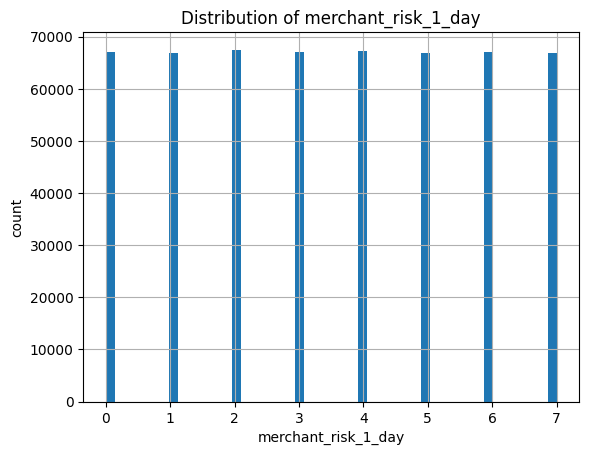
\includegraphics[width=\textwidth]{cell_44_img_05.png}
    \caption{\texttt{merchant\_risk\_1\_day}}
\end{subfigure}
\begin{subfigure}{0.32\textwidth}
    \centering
    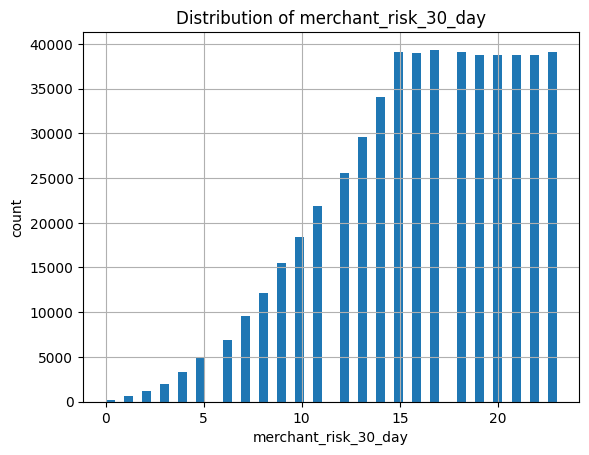
\includegraphics[width=\textwidth]{cell_44_img_06.png}
    \caption{\texttt{merchant\_risk\_30\_day}}
\end{subfigure}
\begin{subfigure}{0.32\textwidth}
    \centering
    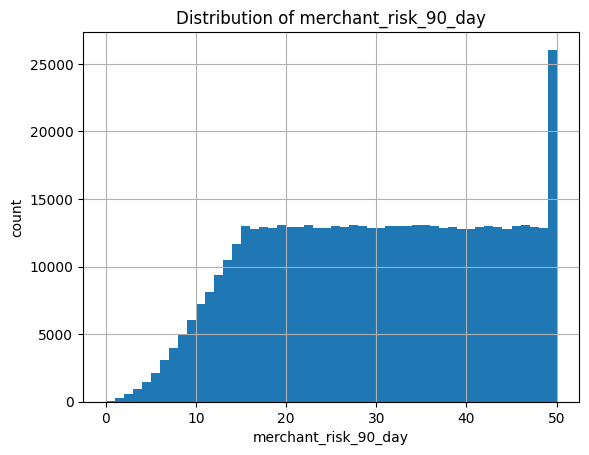
\includegraphics[width=\textwidth]{cell_44_img_07.png}
    \caption{\texttt{merchant\_risk\_90\_day}}
\end{subfigure}
\caption{Merchant risk distributions}
\end{figure}

\begin{figure}[H]
\centering
\begin{subfigure}{0.32\textwidth}
    \centering
    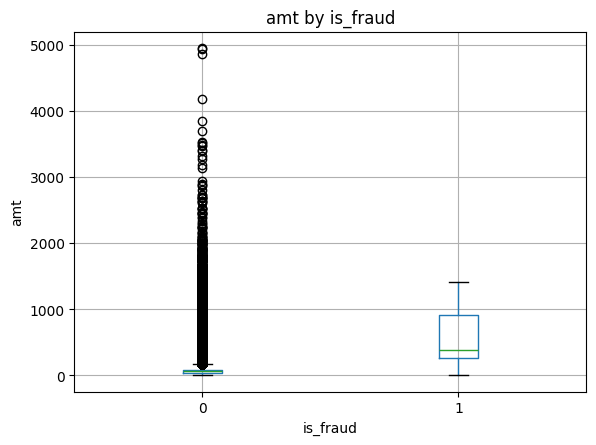
\includegraphics[width=\textwidth]{cell_46_img_01.png}
    \caption{\texttt{amt}}
\end{subfigure}
\begin{subfigure}{0.32\textwidth}
    \centering
    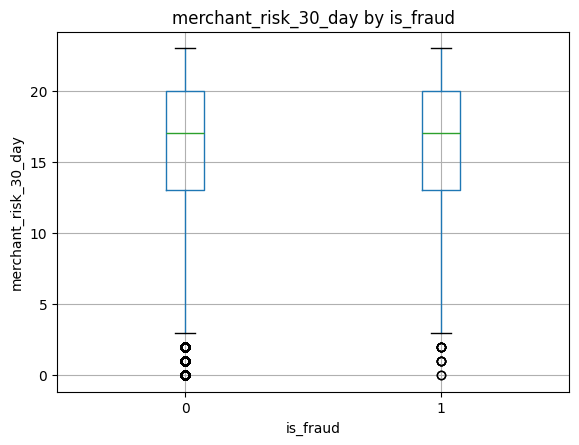
\includegraphics[width=\textwidth]{cell_46_img_02.png}
    \caption{\texttt{merchant\_risk\_30\_day}}
\end{subfigure}
\begin{subfigure}{0.32\textwidth}
    \centering
    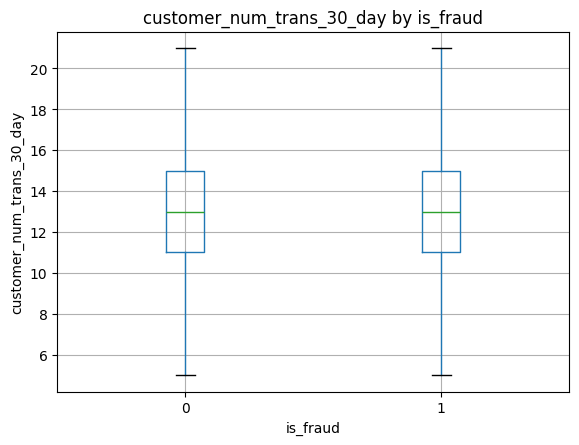
\includegraphics[width=\textwidth]{cell_46_img_03.png}
    \caption{\texttt{customer\_num\_trans\_30\_day}}
\end{subfigure}
\caption{Boxplots by target}
\end{figure}

\begin{figure}[H]
\centering
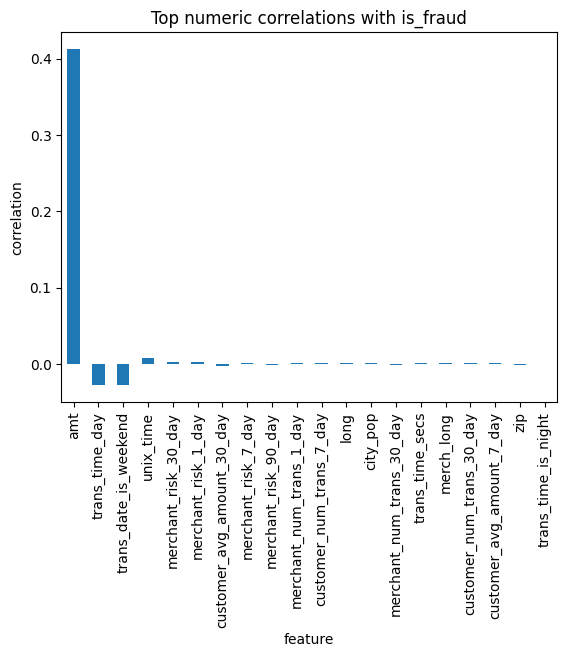
\includegraphics[width=0.75\textwidth]{cell_48_img_01.png}
\caption{Top numeric correlations with fraud label}
\end{figure}

\subsection{Geographic Distance Analysis}

The distance between the customer and merchant is computed using the Haversine formula. The distribution is almost identical for fraud and non-fraud classes.

\begin{table}[H]
\centering
\caption{Customer--merchant distance by class}
\begin{tabular}{lrrr}
\toprule
\textbf{Class} & \textbf{Mean km} & \textbf{Median km} & \textbf{Std km} \\
\midrule
Non-fraud & 76.55 & 78.73 & 29.21 \\
Fraud & 76.77 & 78.60 & 29.34 \\
\bottomrule
\end{tabular}
\end{table}

\begin{figure}[H]
\centering
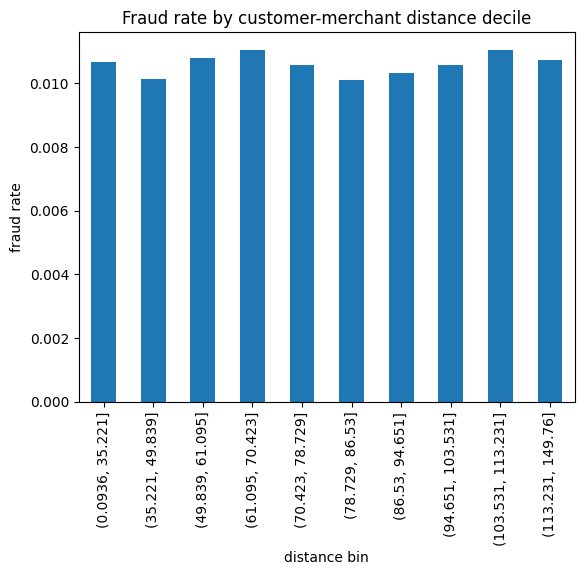
\includegraphics[width=0.70\textwidth]{cell_51_img_01.png}
\caption{Fraud rate by distance decile}
\end{figure}

The fraud rate is nearly flat across distance bins. Therefore, \texttt{customer\_merchant\_distance\_km}, \texttt{merch\_lat}, and \texttt{merch\_long} are not retained in the final feature set.

% ============================================================
\section{Methodology}
% ============================================================

\subsection{Feature Engineering}

The feature engineering process converts raw transaction data into model-ready numerical features. Gender is encoded as a binary variable. Category is one-hot encoded due to its low cardinality. Merchant and job are frequency-encoded because their cardinalities are high. Age is converted into ordinal age bins. Additional ratio features are created, including the current amount relative to the customer's 30-day average amount.

The final transformed dataset contains no remaining object columns and has 43 columns before train/test splitting. After sorting by \texttt{unix\_time}, chunk 01 is split into 429,012 training rows and 107,254 test rows.

\subsection{Feature Selection}

Feature selection uses two complementary approaches: Mutual Information and RandomForest feature importance. A feature is kept if it appears in the top-20 of either ranking, after removing highly collinear drop candidates.

\begin{figure}[H]
\centering
\begin{subfigure}{0.48\textwidth}
    \centering
    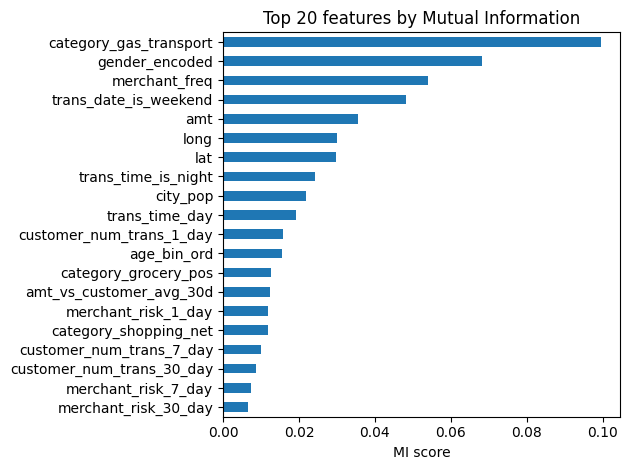
\includegraphics[width=\textwidth]{cell_60_img_01.png}
    \caption{Mutual Information}
\end{subfigure}
\begin{subfigure}{0.48\textwidth}
    \centering
    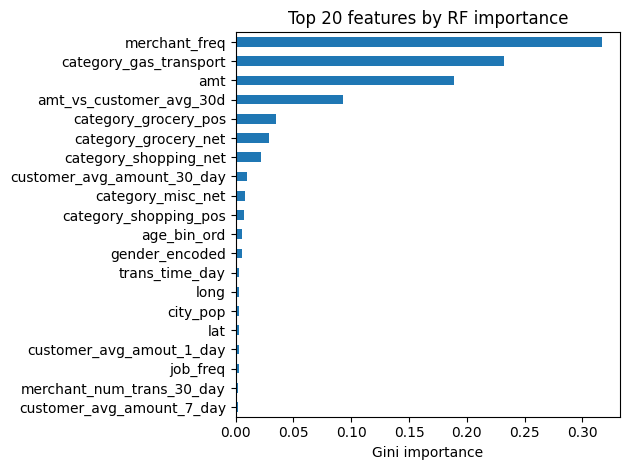
\includegraphics[width=\textwidth]{cell_62_img_01.png}
    \caption{RandomForest importance}
\end{subfigure}
\caption{Feature ranking plots}
\end{figure}

\begin{table}[H]
\centering
\caption{Feature selection impact}
\begin{tabular}{lrr}
\toprule
\textbf{Feature set} & \textbf{Number of features} & \textbf{PR-AUC} \\
\midrule
All model-ready features & 41 & 0.9588 \\
Selected features & 25 & 0.9576 \\
\midrule
Difference & -16 & -0.0013 \\
\bottomrule
\end{tabular}
\end{table}

The selected feature set reduces dimensionality by 39\% while losing only 0.0013 PR-AUC. This indicates that many features are redundant or weak, and a smaller feature set can improve robustness and reduce training cost.

\subsection{Handling Imbalanced Data}

Two imbalance-handling strategies are compared for XGBoost:
\begin{itemize}
    \item \textbf{Class weighting}: keep the original data distribution and use \texttt{scale\_pos\_weight}.
    \item \textbf{Undersampling}: reduce the majority class to a 10:1 negative-to-positive ratio.
\end{itemize}

Class weighting is preferred for the final recommendation because it preserves the original distribution and is more stable across future chunks.

\subsection{Modeling Approach}

The notebook evaluates RandomForest and XGBoost variants with baseline, class-weighted, and undersampled strategies. XGBoost provides the strongest validation PR-AUC and is selected for hyperparameter tuning.

\begin{table}[H]
\centering
\caption{Initial model and imbalance-strategy comparison on chunk 01}
\begin{tabular}{llrr}
\toprule
\textbf{Name} & \textbf{Strategy} & \textbf{Train size} & \textbf{Validation PR-AUC} \\
\midrule
rf\_baseline & baseline & 343,209 & 0.9417 \\
rf\_class\_weight & class weight & 343,209 & 0.9444 \\
rf\_undersample & undersample & 39,886 & 0.9587 \\
xgb\_baseline & baseline & 343,209 & 0.9655 \\
xgb\_class\_weight & class weight & 343,209 & 0.9655 \\
xgb\_undersample & undersample & 39,886 & 0.9724 \\
\bottomrule
\end{tabular}
\end{table}

% ============================================================
\section{Experiments, Evaluation, and Results}
% ============================================================

\subsection{Evaluation Strategy}

The project uses PR-AUC for model ranking and F1-score for threshold-based classification quality. Accuracy is excluded from the main analysis because the dataset is severely imbalanced. For threshold tuning, the validation Precision--Recall curve is used to select the threshold that maximizes F1:
\begin{equation}
    \tau^* = \arg\max_{\tau} F1(y_{\text{val}}, \hat{p}_{\text{val}} \ge \tau).
\end{equation}

The selected threshold is then applied to the test set.

\subsection{Hyperparameter Tuning}

The top two XGBoost candidates are tuned with Optuna using validation PR-AUC as the objective.

\begin{table}[H]
\centering
\caption{Best tuned XGBoost hyperparameters}
\resizebox{\textwidth}{!}{
\begin{tabular}{lrrrrrrrrr}
\toprule
\textbf{Model} & \textbf{n\_est} & \textbf{depth} & \textbf{lr} & \textbf{subsample} & \textbf{colsample} & \textbf{child} & \textbf{alpha} & \textbf{lambda} & \textbf{gamma} \\
\midrule
xgb\_undersample & 150 & 8 & 0.016664 & 0.948150 & 0.781684 & 6 & 0.189588 & 0.007976 & 0.660841 \\
xgb\_class\_weight & 400 & 6 & 0.015384 & 0.880095 & 0.754347 & 1 & 0.155126 & 0.005929 & 3.799895 \\
\bottomrule
\end{tabular}
}
\end{table}

\subsection{Chunk 01 Final Evaluation}

Both tuned XGBoost models perform strongly on chunk 01 test data.

\begin{table}[H]
\centering
\caption{Final tuned model results on chunk 01 test set}
\begin{tabular}{lrrrrrrr}
\toprule
\textbf{Model} & \textbf{PR-AUC} & \textbf{Threshold} & \textbf{F1} & \textbf{TN} & \textbf{FP} & \textbf{FN} & \textbf{TP} \\
\midrule
xgb\_undersample & 0.9614 & 0.7484 & 0.9564 & 106,356 & 0 & 75 & 823 \\
xgb\_class\_weight & 0.9623 & 0.9722 & 0.9564 & 106,356 & 0 & 75 & 823 \\
\bottomrule
\end{tabular}
\end{table}

For the fraud class, both final models reach precision 1.0000 and recall 0.9165 on chunk 01 test data. This means that, in this test segment, the models do not produce false positive alerts at the selected thresholds, while still detecting 823 out of 898 fraud cases.

\begin{figure}[H]
\centering
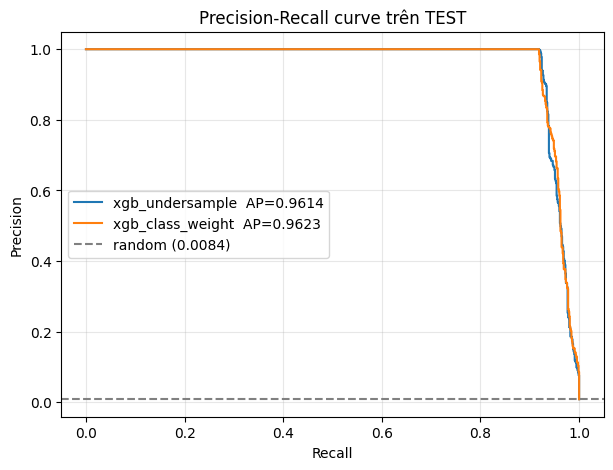
\includegraphics[width=0.70\textwidth]{cell_88_img_01.png}
\caption{Precision--Recall curve of tuned XGBoost models on chunk 01}
\end{figure}

\subsection{Cross-Chunk Evaluation}

The chunk 01 result is strong, but a production model must generalize to later time periods. Therefore, the tuned parameters are applied to chunks 02--16. Chunk 16 is excluded from quality conclusions because its test segment contains no fraud cases.

\begin{table}[H]
\centering
\caption{Mean cross-chunk performance excluding no-positive test chunks}
\begin{tabular}{lrrr}
\toprule
\textbf{Model} & \textbf{Mean test PR-AUC} & \textbf{Mean F1 at validation threshold} & \textbf{Best diagnostic F1} \\
\midrule
xgb\_class\_weight & 0.8025 & 0.6031 & 0.7935 \\
xgb\_undersample & 0.7736 & 0.5957 & 0.7814 \\
\bottomrule
\end{tabular}
\end{table}

\begin{figure}[H]
\centering
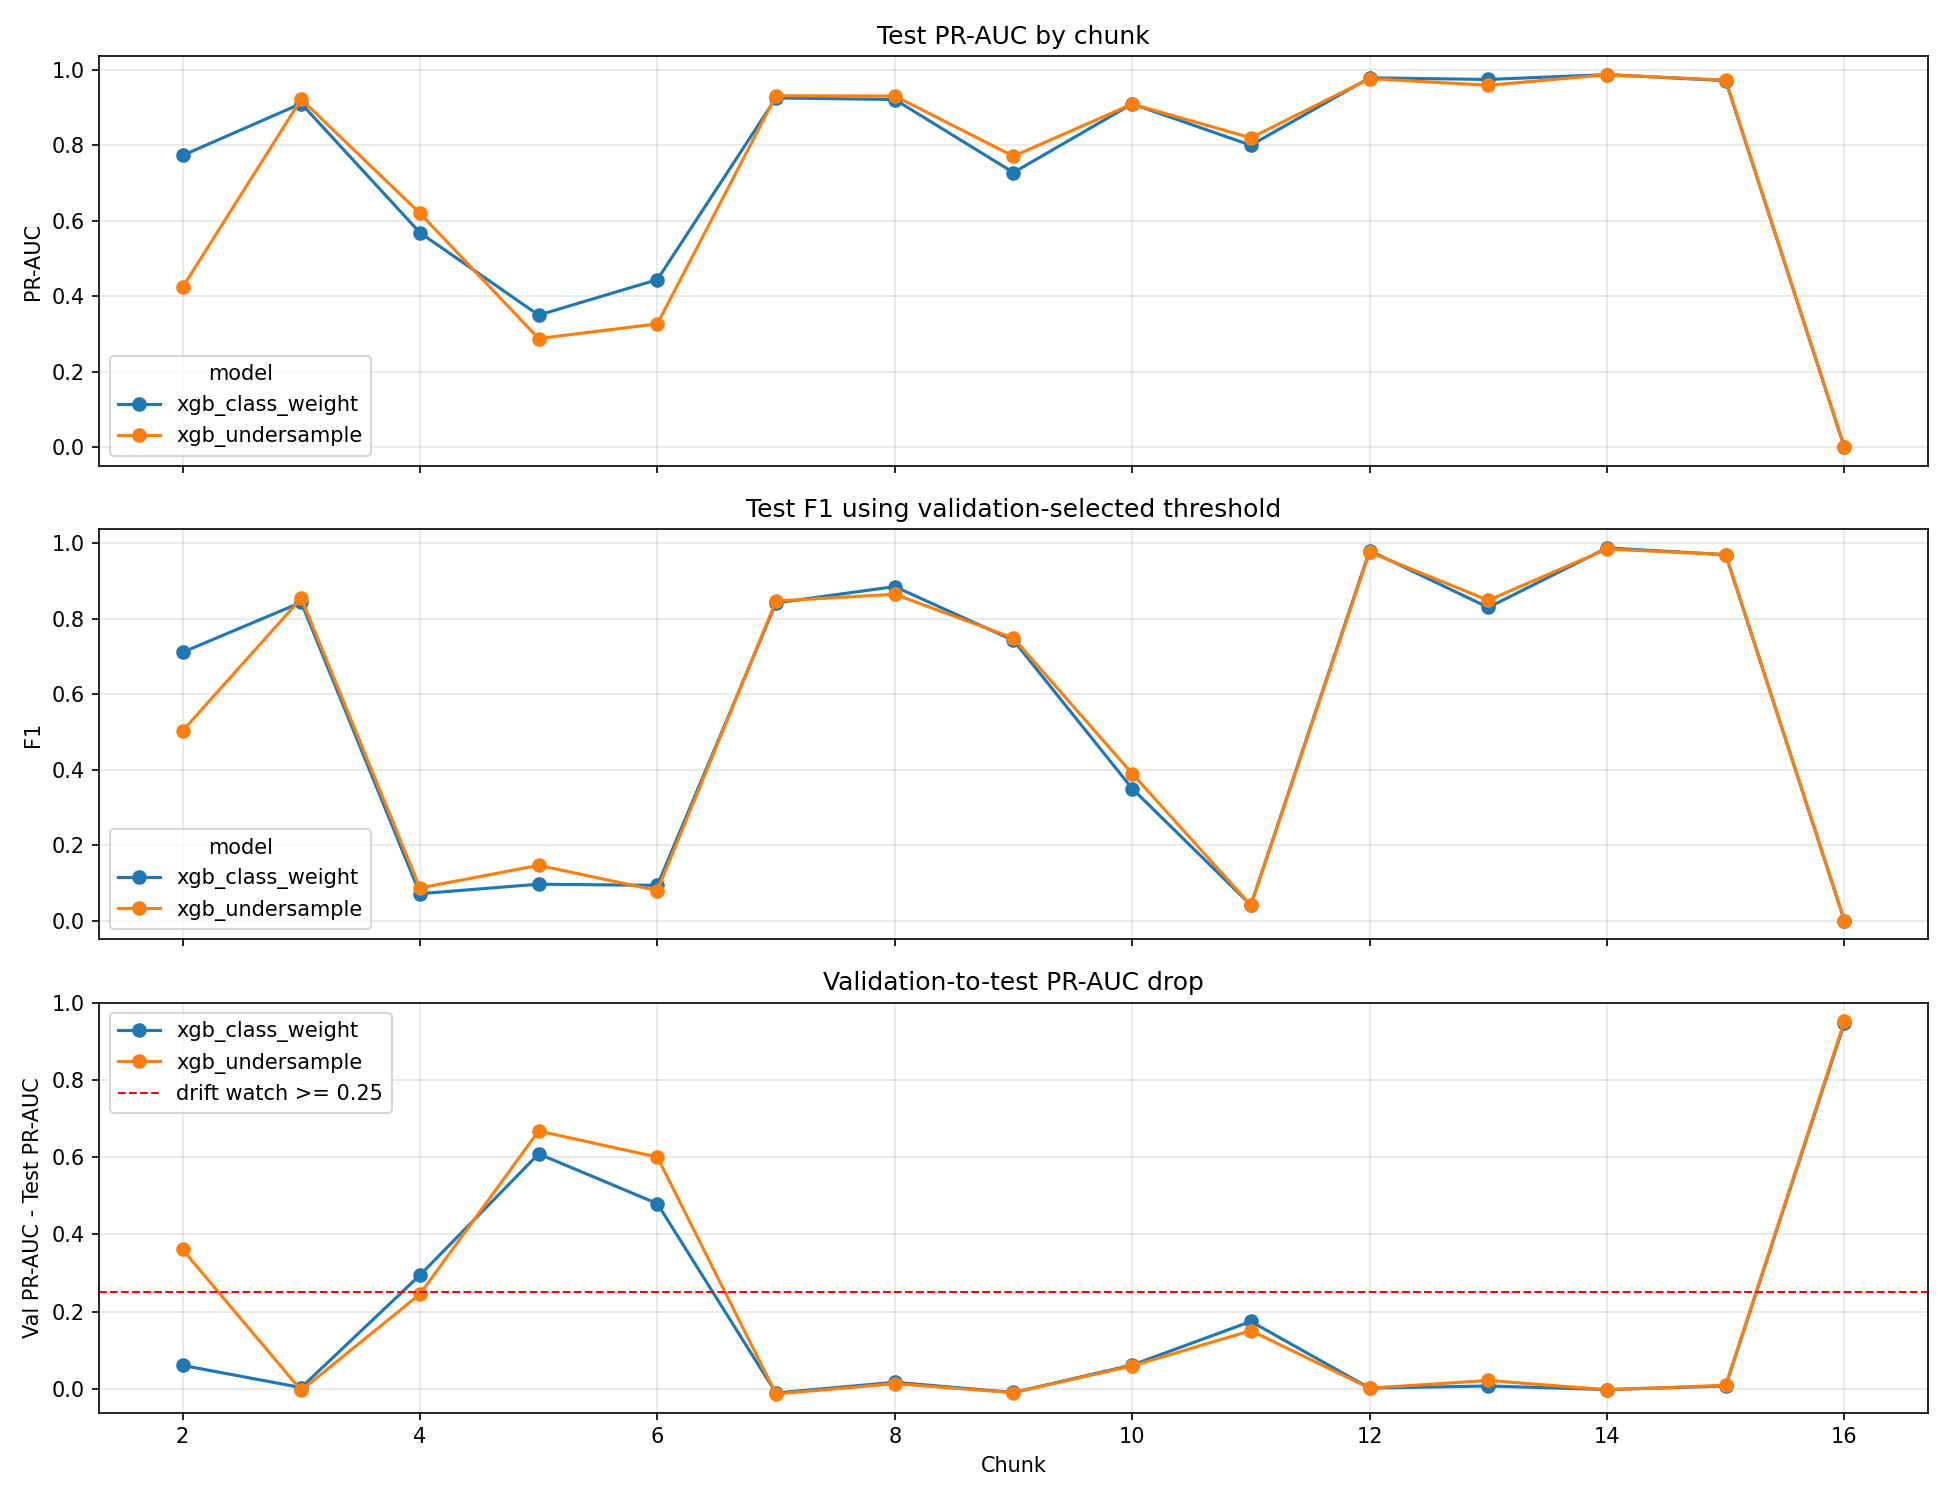
\includegraphics[width=\textwidth]{xgb_chunks_02_16_drift_aware_metrics.png}
\caption{Chunk-level PR-AUC, F1, and validation-to-test PR-AUC drop}
\end{figure}

The cross-chunk results show that strong performance on chunk 01 does not guarantee stable performance on future chunks. The average PR-AUC decreases substantially when evaluating across later chunks.

% ============================================================
\section{Drift Analysis}
% ============================================================

\subsection{Separating Concept Drift and Threshold Drift}

Low F1-score alone is not sufficient evidence of concept drift. The report separates two possible failure modes:
\begin{itemize}
    \item \textbf{Ranking/concept drift}: PR-AUC drops strongly, meaning the model no longer ranks fraud above non-fraud reliably.
    \item \textbf{Threshold drift}: PR-AUC remains high, but F1-score becomes low because the validation threshold no longer matches the test score distribution.
\end{itemize}

\begin{table}[H]
\centering
\caption{Diagnosis of selected low-F1 chunks using \texttt{xgb\_class\_weight}}
\begin{tabular}{crrrl}
\toprule
\textbf{Chunk} & \textbf{Val PR-AUC} & \textbf{Test PR-AUC} & \textbf{F1 at val threshold} & \textbf{Diagnosis} \\
\midrule
2 & 0.8338 & 0.7726 & 0.7109 & OK \\
4 & 0.8629 & 0.5682 & 0.0715 & Ranking drift suspected \\
5 & 0.9586 & 0.3500 & 0.0966 & Concept/label drift likely \\
6 & 0.9238 & 0.4439 & 0.0935 & Concept/label drift likely \\
9 & 0.7184 & 0.7274 & 0.7427 & OK \\
10 & 0.9712 & 0.9091 & 0.3500 & Threshold calibration drift \\
11 & 0.9745 & 0.7997 & 0.0414 & Threshold calibration drift \\
\bottomrule
\end{tabular}
\end{table}

\subsection{Concept or Label Drift Candidates}

Chunks 5 and 6 are the strongest concept or label drift candidates. Their validation PR-AUC values are high, but their test PR-AUC values collapse to 0.3500 and 0.4439 respectively. Even the best diagnostic test F1 remains low. This suggests that the model is not only miscalibrated; it is no longer ranking fraud reliably in those test segments.

\subsection{Threshold Calibration Drift}

Chunks 10 and 11 behave differently. Their test PR-AUC values remain relatively high, but their F1-scores at validation-selected thresholds are very low. The best diagnostic F1 values are much higher, indicating that the model still ranks fraud well but the threshold is no longer appropriate.

\begin{figure}[H]
\centering
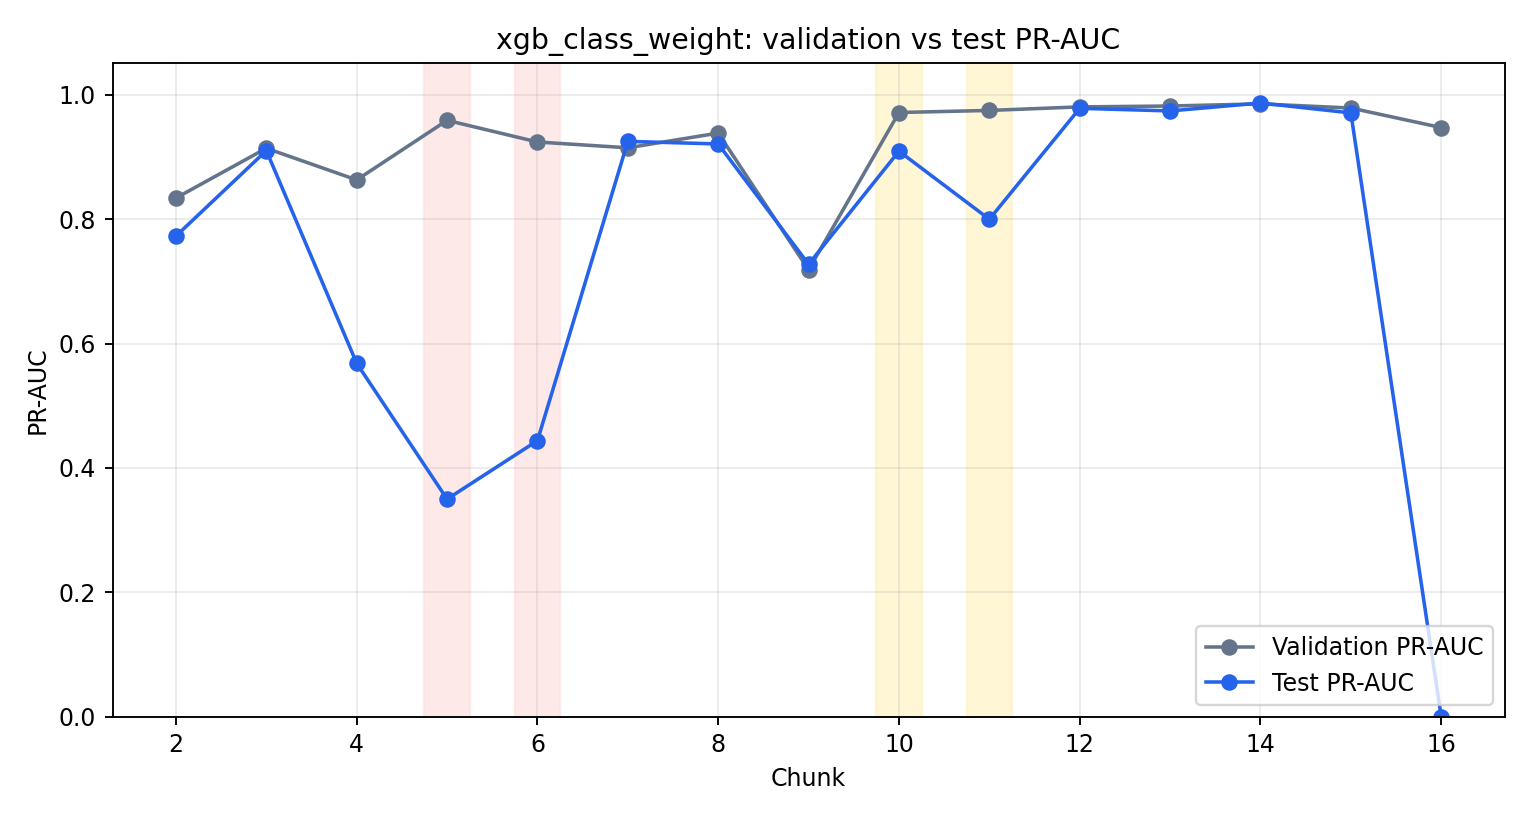
\includegraphics[width=0.85\textwidth]{class_weight_val_test_pr_auc.png}
\caption{Validation vs test PR-AUC for \texttt{xgb\_class\_weight}}
\end{figure}

\begin{figure}[H]
\centering
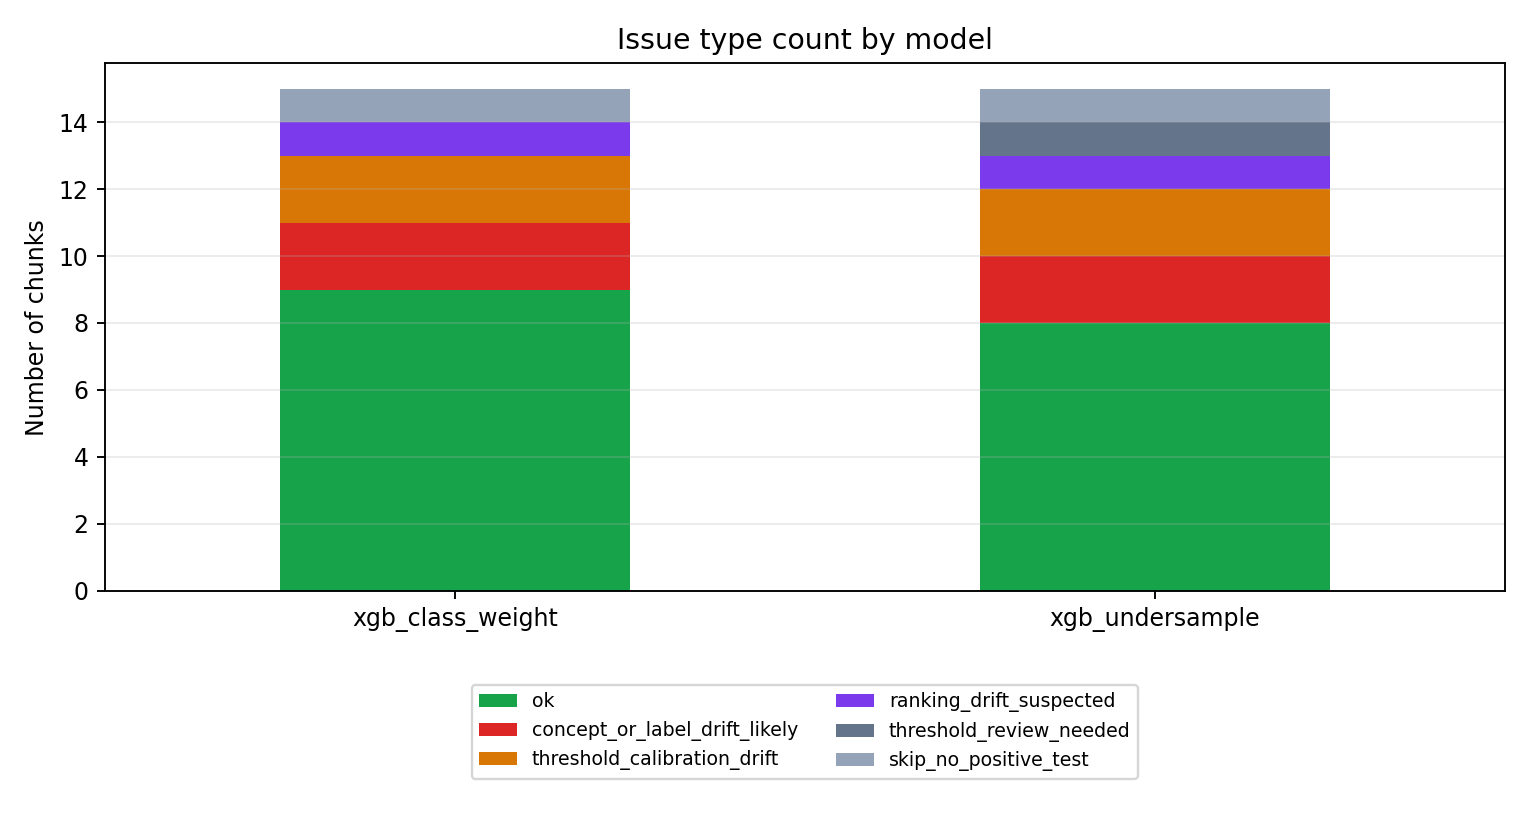
\includegraphics[width=0.85\textwidth]{issue_type_counts.png}
\caption{Issue type counts across chunks 02--16}
\end{figure}

This distinction is operationally important. If a chunk suffers from threshold drift, the system should recalibrate the threshold before retraining the entire model. If a chunk suffers from ranking or concept drift, retraining with a more recent rolling window becomes more appropriate.

% ============================================================
\section{Deployment Plan}
% ============================================================

\subsection{Recommended Pipeline}

Based on the full analysis, the recommended pipeline is:
\begin{enumerate}
    \item Use the selected 25-feature set.
    \item Use XGBoost with class weighting as the production baseline.
    \item Use time-based walk-forward validation.
    \item Select thresholds dynamically using the most recent validation window.
    \item Monitor PR-AUC, F1-score, fraud rate, and feature distribution drift.
    \item Retrain only when ranking quality degrades, not merely when F1-score drops.
\end{enumerate}

\subsection{Inference Contract}

The inference pipeline should require the same feature order used during training. Raw inputs must be transformed into the selected model features, including amount ratios, age bins, category one-hot features, frequency encodings, rolling customer behavior, and merchant risk features. The model should output both a fraud probability and a binary decision based on the current operating threshold.

\subsection{Monitoring}

Monitoring should distinguish between model ranking degradation and threshold instability. Recommended monitoring indicators include:
\begin{itemize}
    \item PR-AUC and F1-score over time.
    \item Fraud rate by time window.
    \item False positive and false negative counts.
    \item PSI or KS statistics for important features such as \texttt{amt}, category indicators, \texttt{merchant\_freq}, \texttt{job\_freq}, and rolling behavior features.
    \item Difference between validation PR-AUC and future test PR-AUC.
\end{itemize}

% ============================================================
\section{Conclusion and Future Work}
% ============================================================

\subsection{Executive Summary}

The project shows that XGBoost is highly effective for credit card fraud detection on the analyzed tabular dataset. Chunk 01 results are very strong, with PR-AUC above 0.96 and F1-score above 0.95. EDA shows that amount and category are the strongest signals, while distance and time-of-day are weak standalone signals. Feature selection reduces the number of model features from 41 to 25 with almost no PR-AUC loss.

However, cross-chunk evaluation reveals that the model is not uniformly stable over time. Chunks 5 and 6 show evidence of concept or label drift, while chunks 10 and 11 mainly show threshold calibration drift. Therefore, a realistic fraud detection system should not rely on a single static threshold or a single validation split.

The final recommendation is to use \texttt{xgb\_class\_weight} with the selected feature set, dynamic thresholding, walk-forward validation, and drift-aware monitoring.

\subsection{Limitations}

Several limitations remain:
\begin{itemize}
    \item Some category patterns appear nearly deterministic in chunk 01 and may reflect dataset artifacts.
    \item Frequency encoding was computed within the analysis pipeline and should be adapted carefully for production.
    \item The dataset is synthetic or simulation-based, so real production data may contain additional noise.
    \item The report does not implement an online learning system; it only proposes a monitoring and retraining strategy.
\end{itemize}

\subsection{Future Work}

Future work should focus on:
\begin{itemize}
    \item Implementing walk-forward training using rolling windows.
    \item Adding probability calibration methods such as Platt scaling or isotonic calibration.
    \item Testing cost-based threshold optimization instead of F1-only thresholding.
    \item Building a production-ready inference API.
    \item Extending drift detection with PSI, KS-test, and label-delay-aware monitoring.
\end{itemize}

% ============================================================
\begin{thebibliography}{9}
\addcontentsline{toc}{section}{References}

\bibitem{xgboost}
T. Chen and C. Guestrin.
\textit{XGBoost: A Scalable Tree Boosting System}.
Proceedings of the 22nd ACM SIGKDD International Conference on Knowledge Discovery and Data Mining, 2016.

\bibitem{randomforest}
L. Breiman.
\textit{Random Forests}.
Machine Learning, 45(1), 5--32, 2001.

\bibitem{smote}
N. V. Chawla, K. W. Bowyer, L. O. Hall, and W. P. Kegelmeyer.
\textit{SMOTE: Synthetic Minority Over-sampling Technique}.
Journal of Artificial Intelligence Research, 16, 321--357, 2002.

\bibitem{sklearn}
F. Pedregosa et al.
\textit{Scikit-learn: Machine Learning in Python}.
Journal of Machine Learning Research, 12, 2825--2830, 2011.

\bibitem{optuna}
T. Akiba, S. Sano, T. Yanase, T. Ohta, and M. Koyama.
\textit{Optuna: A Next-generation Hyperparameter Optimization Framework}.
Proceedings of the 25th ACM SIGKDD International Conference, 2019.

\end{thebibliography}

\end{document}
